%%%%%%%%%%%%%%%%%%%%%%%%%%%%%%%%%%%%%%%%%
% Beamer Presentation
% LaTeX Template
% Version 2.0 (March 8, 2022)
%
% This template originates from:
% https://www.LaTeXTemplates.com
%
% Author:
% Vel (vel@latextemplates.com)
%
% License:
% CC BY-NC-SA 4.0 (https://creativecommons.org/licenses/by-nc-sa/4.0/)
%
%%%%%%%%%%%%%%%%%%%%%%%%%%%%%%%%%%%%%%%%%

%----------------------------------------------------------------------------------------
%	PACKAGES AND OTHER DOCUMENT CONFIGURATIONS
%----------------------------------------------------------------------------------------

\documentclass[
	11pt, % Set the default font size, options include: 8pt, 9pt, 10pt, 11pt, 12pt, 14pt, 17pt, 20pt
	%t, % Uncomment to vertically align all slide content to the top of the slide, rather than the default centered
	%aspectratio=169, % Uncomment to set the aspect ratio to a 16:9 ratio which matches the aspect ratio of 1080p and 4K screens and projectors
]{beamer}

\graphicspath{{Images/}{./}} % Specifies where to look for included images (trailing slash required)

\usepackage{booktabs} % Allows the use of \toprule, \midrule and \bottomrule for better rules in tables
\usepackage{graphicx}
\usepackage{amsmath}
\usepackage{amssymb}
\usepackage{mathtools}
\usepackage{amsthm}
\usepackage{biblatex}
%\addbibresource{presentation.bib}
%----------------------------------------------------------------------------------------
%	SELECT LAYOUT THEME
%----------------------------------------------------------------------------------------

% Beamer comes with a number of default layout themes which change the colors and layouts of slides. Below is a list of all themes available, uncomment each in turn to see what they look like.

\usetheme{Madrid}


%----------------------------------------------------------------------------------------
%	SELECT FONT THEME & FONTS
%----------------------------------------------------------------------------------------

% Beamer comes with several font themes to easily change the fonts used in various parts of the presentation. Review the comments beside each one to decide if you would like to use it. Note that additional options can be specified for several of these font themes, consult the beamer documentation for more information.

\usefonttheme{default} % Typeset using the default sans serif font

%------------------------------------------------

%\usepackage{mathptmx} % Use the Times font for serif text
%\usepackage{palatino} % Use the Palatino font for serif text

%\usepackage{helvet} % Use the Helvetica font for sans serif text
\usepackage[default]{opensans} % Use the Open Sans font for sans serif text
%\usepackage[default]{FiraSans} % Use the Fira Sans font for sans serif text
%\usepackage[default]{lato} % Use the Lato font for sans serif text

%----------------------------------------------------------------------------------------
%	SELECT INNER THEME
%----------------------------------------------------------------------------------------

% Inner themes change the styling of internal slide elements, for example: bullet points, blocks, bibliography entries, title pages, theorems, etc. Uncomment each theme in turn to see what changes it makes to your presentation.

%\useinnertheme{default}
\useinnertheme{circles}
%\useinnertheme{rectangles}
%\useinnertheme{rounded}
%\useinnertheme{inmargin}

%----------------------------------------------------------------------------------------
%	SELECT OUTER THEME
%----------------------------------------------------------------------------------------

% Outer themes change the overall layout of slides, such as: header and footer lines, sidebars and slide titles. Uncomment each theme in turn to see what changes it makes to your presentation.

%\useoutertheme{default}
%\useoutertheme{infolines}
%\useoutertheme{miniframes}
%\useoutertheme{smoothbars}
%\useoutertheme{sidebar}
%\useoutertheme{split}
%\useoutertheme{shadow}
%\useoutertheme{tree}
%\useoutertheme{smoothtree}

%\setbeamertemplate{footline} % Uncomment this line to remove the footer line in all slides
%\setbeamertemplate{footline}[page number] % Uncomment this line to replace the footer line in all slides with a simple slide count

%\setbeamertemplate{navigation symbols}{} % Uncomment this line to remove the navigation symbols from the bottom of all slides

%----------------------------------------------------------------------------------------
%	PRESENTATION INFORMATION
%----------------------------------------------------------------------------------------

\title[ESG]{Extremum Seeking Gradient} % The short title in the optional parameter appears at the bottom of every slide, the full title in the main parameter is only on the title page

\subtitle{Machine Learning without Backpropagation} % Presentation subtitle, remove this command if a subtitle isn't required

\author[Prichen, Dicker]{David Prichen \and Or Dicker} % Presenter name(s), the optional parameter can contain a shortened version to appear on the bottom of every slide, while the main parameter will appear on the title slide

\institute[TAU]{Tel Aviv University} % Your institution, the optional parameter can be used for the institution shorthand and will appear on the bottom of every slide after author names, while the required parameter is used on the title slide and can include your email address or additional information on separate lines

\date[]{Project Day - 0510725502 \\ \today} % Presentation date or conference/meeting name, the optional parameter can contain a shortened version to appear on the bottom of every slide, while the required parameter value is output to the title slide

%----------------------------------------------------------------------------------------

\begin{document}

%----------------------------------------------------------------------------------------
%	TITLE SLIDE
%----------------------------------------------------------------------------------------

\begin{frame}
	\titlepage % Output the title slide, automatically created using the text entered in the PRESENTATION INFORMATION block above
\end{frame}


%----------------------------------------------------------------------------------------
%	PRESENTATION BODY SLIDES
%----------------------------------------------------------------------------------------


\begin{frame}
  \frametitle{What's is wrong with backpropagation}
  \begin{itemize}
  \item Not biologically plausible
    \begin{itemize}
    \item Neurons cannot store input values for a future
      backward pass
      \item Neurons do not wait for signals to pass through the
entire brain to update connections
\end{itemize}
\item Requires perfect knowledge of forward pass
  \begin{itemize}
\item Can only improve weights of one layer if we have total
knowledge of forward and backward pass
\end{itemize}
\item Typically, specialized chips designed for neural networks are unable to execute the backpropagation process.
\end{itemize}
\end{frame}

%------------------------------------------------

\begin{frame}
  \frametitle{Example of Photonic Neural Network}
    Experimentally realized in situ backpropagation for deep learning in nanophotonic
neural networks (Nature paper)
  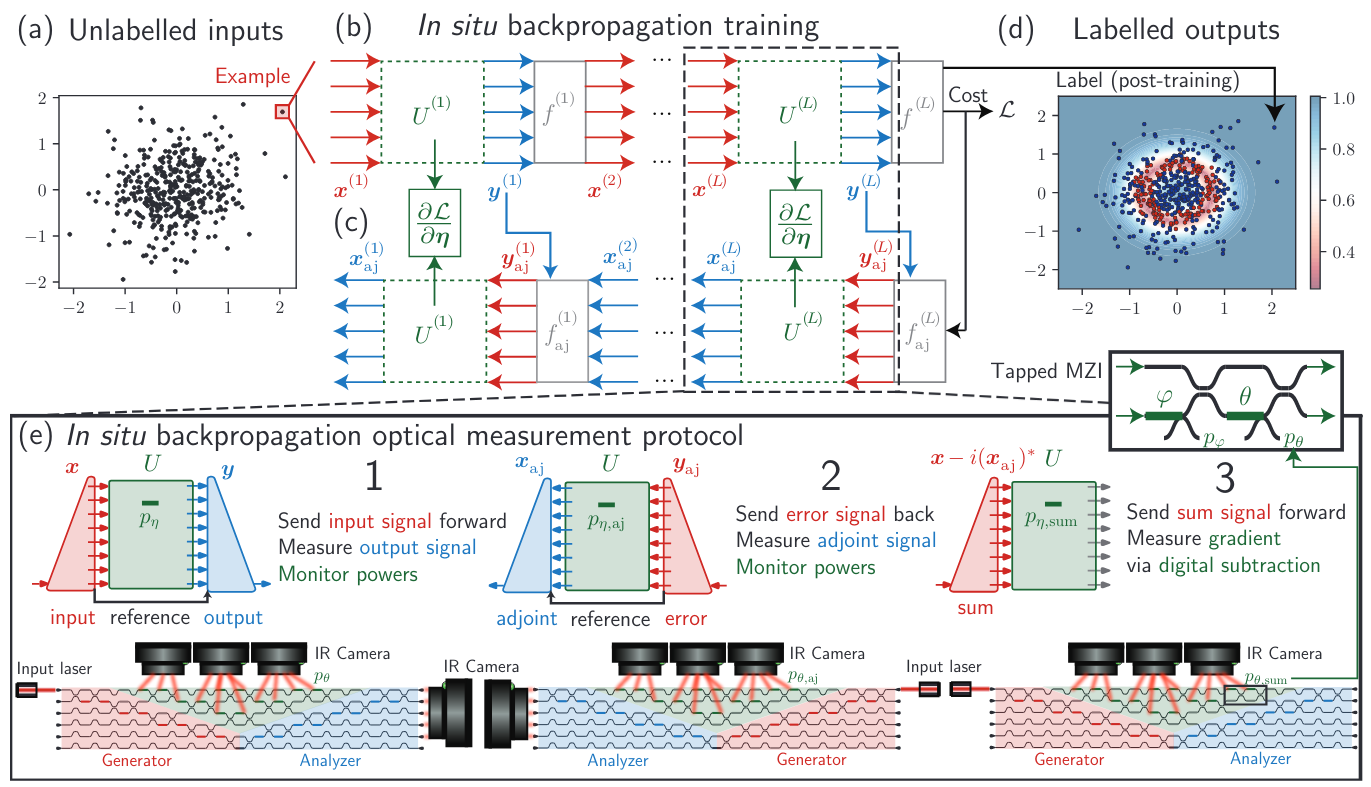
\includegraphics[width=0.8\columnwidth]{../report/images/photonic_nn.png}
\end{frame}

%------------------------------------------------


\begin{frame}
  \frametitle{Forward Forward Algorithm by Geoffrey Hinton}
  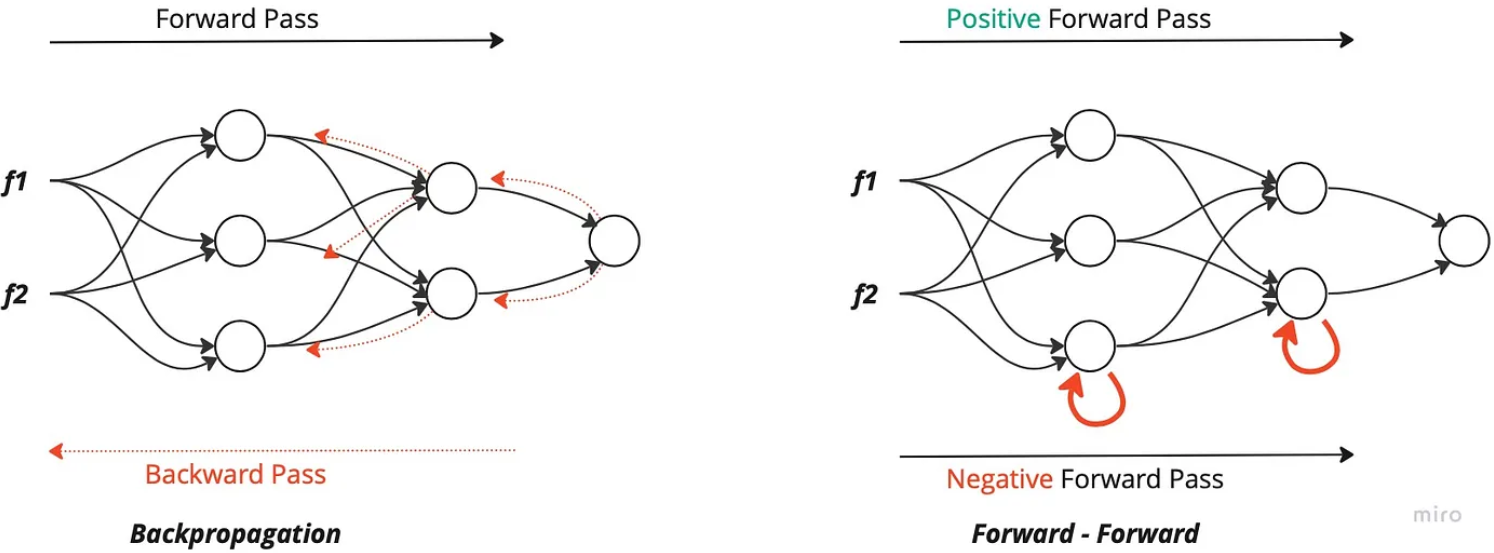
\includegraphics[width=\columnwidth]{../report/images/FF_scheme.png}
\end{frame}

%------------------------------------------------

\begin{frame}
  \frametitle{Spectrum of Learning Algorithms}
  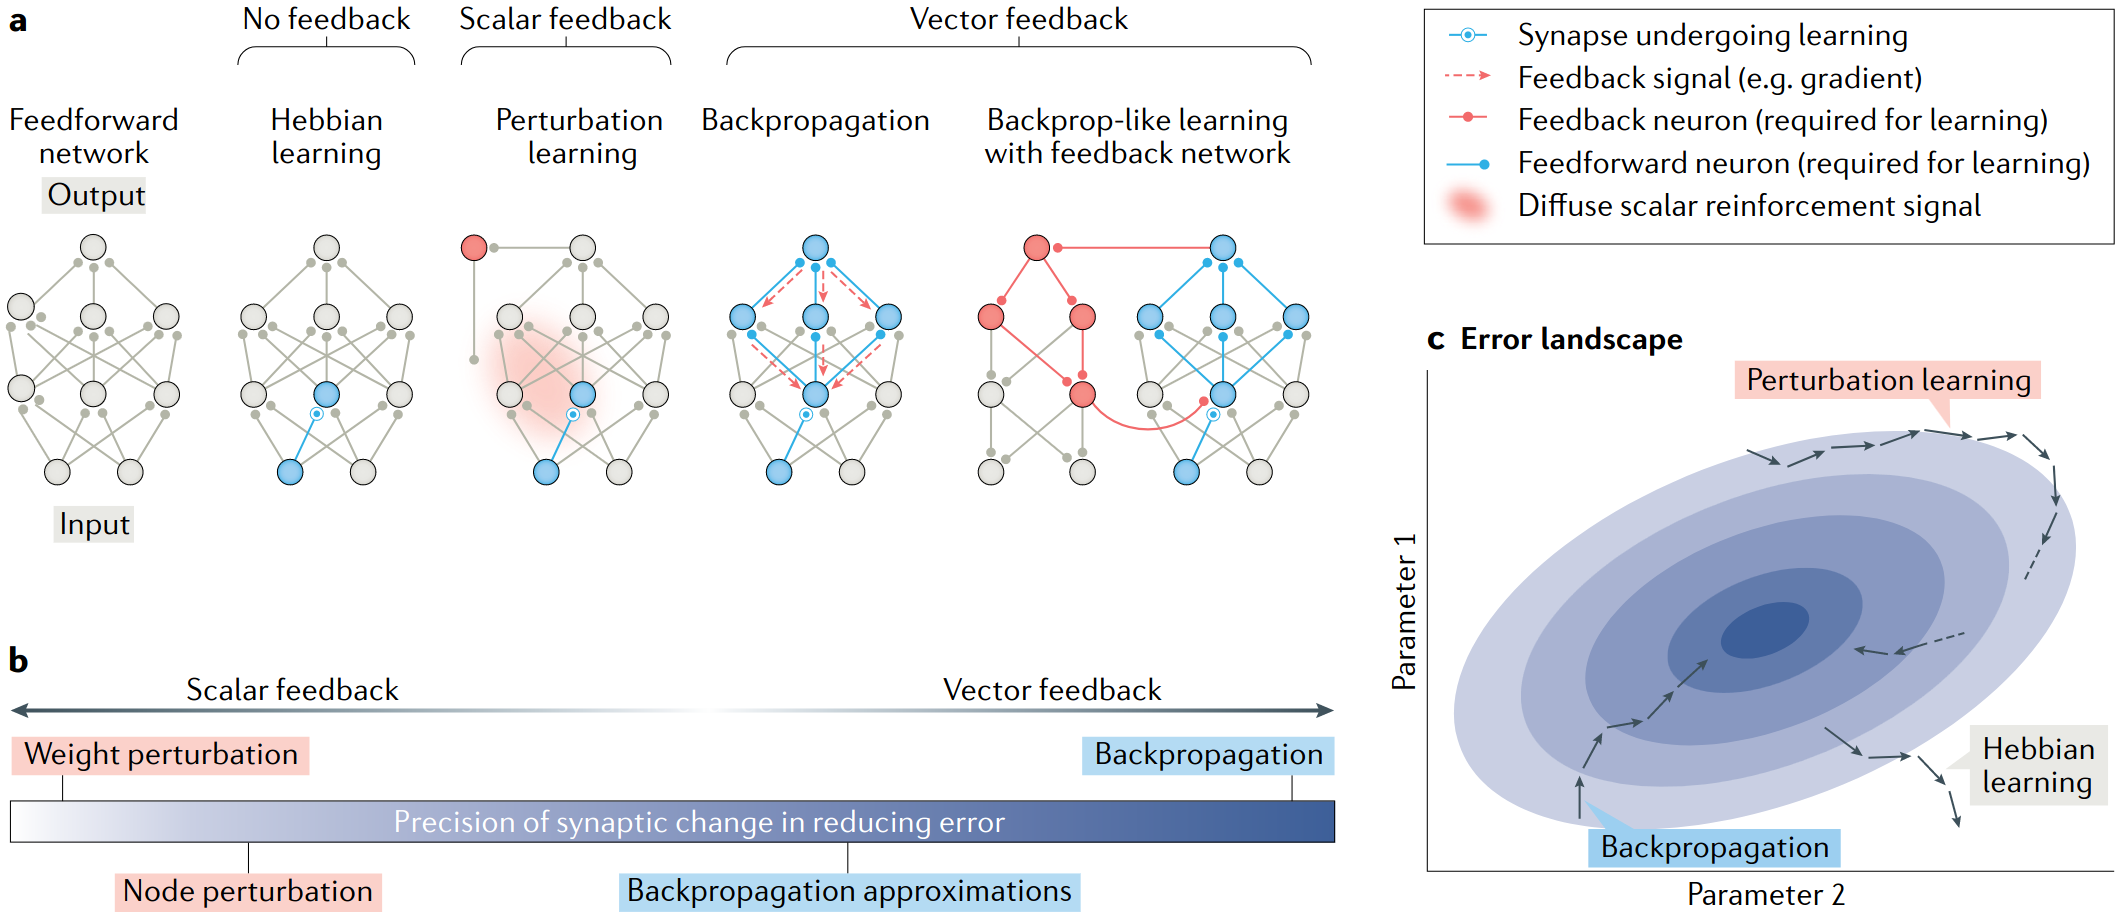
\includegraphics[width=\columnwidth]{../report/images/grad_landscape.png}
  We introduce a novel perturbation learning algorithm suitable for application in photonic neural networks
\end{frame}

%------------------------------------------------

\begin{frame}
  \frametitle{Extremum Seeking Control}
   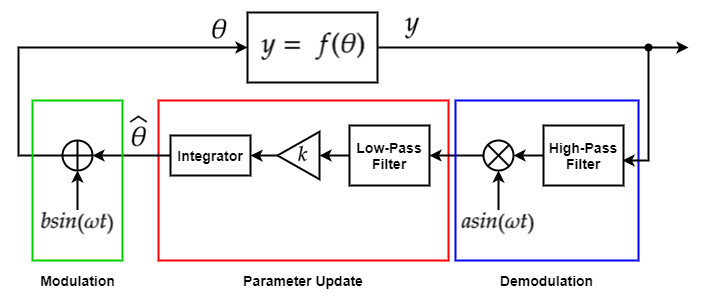
\includegraphics[width=0.9\columnwidth]{../report/images/esc_static_optimization.png}
\end{frame}


%------------------------------------------------

\begin{frame}
  \frametitle{Extremum Seeking Control}
  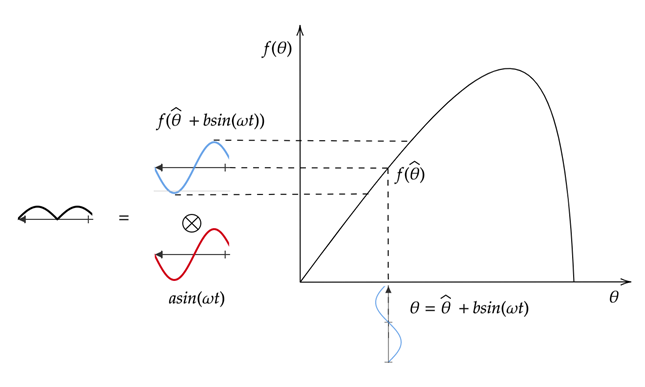
\includegraphics[width=0.9\columnwidth]{../report/images/esc_increasing_objective.png}
\end{frame}


%------------------------------------------------


\begin{frame}
  \frametitle{Extremum Seeking Gradient}
  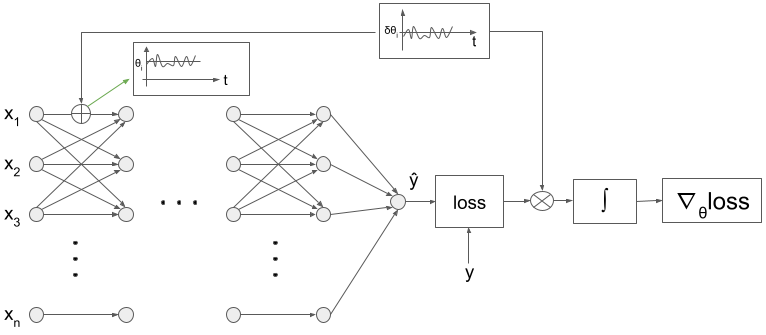
\includegraphics[width=\columnwidth]{../report/images/ESG-scheme.png}
\end{frame}


%------------------------------------------------


\begin{frame}
  \frametitle{Math proof}
  \begin{proof}
    Let's define $\hat{y} \coloneqq NN(x;\theta)$ and $f(\theta) \coloneqq loss(NN(x_{i};\theta),y_{i})$
    where $\theta$ is NN parameters and $\{x_{i},y_{i}\}$ is the dataset. In addition, $E[\delta\theta] = 0$ and $E[\delta\theta \delta\theta^{T}]=\sigma^{2}I$. \newline
    Now, let's evaluate:
    $$E[f(\theta+\delta\theta)\delta\theta]$$
    $$=E[(f(\theta)+\delta\theta^{T} \nabla f(\theta)+O(\delta\theta^{2}))\cdot \delta\theta)] = E[f(\theta)\cdot \delta\theta]+E[\delta\theta^{T} \nabla f(\theta)\cdot \delta\theta]$$
    $$=f(\theta)E[\delta\theta]+E[\delta\theta \delta\theta^{T}] \nabla f(\theta) = \sigma^{2} \nabla f(\theta)$$ 
 \end{proof}


\begin{theorem}[ESG]
$$\nabla f(\theta) \approx \frac{1}{N\sigma^{2}}\sum^{N}_{n=1} f(\theta+\delta\theta)\cdot \delta\theta$$
\end{theorem}



\end{frame}

%------------------------------------------------

\begin{frame}
  \frametitle{Experiments}


      \begin{columns}[c]
% create the column with the first image, that occupies
% half of the slide
    \begin{column}{.5\textwidth}
    \begin{figure}
        \centering
        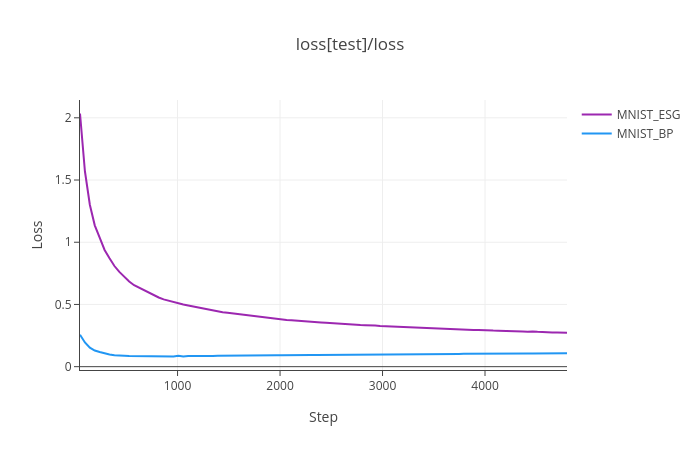
\includegraphics[width=0.7\textwidth]{../report/images/MNIST_test.png}
        \caption{MNIST test}
    \end{figure}      
    \end{column}
% create the column with the second image, that also
% occupies half of the slide
    \begin{column}{.5\textwidth}
    \begin{figure}
        \centering
        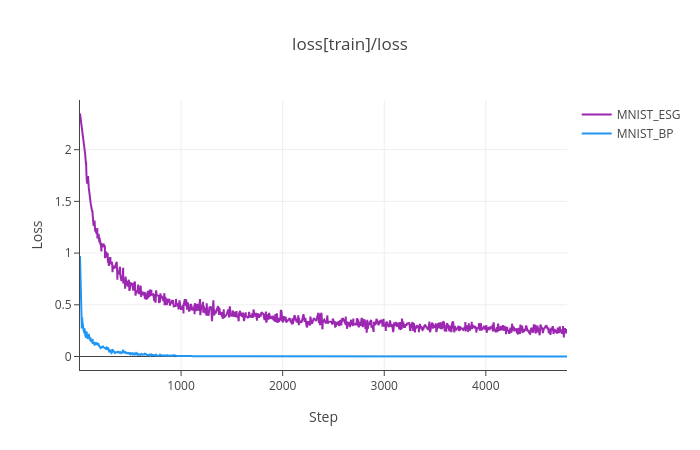
\includegraphics[width=0.7\textwidth]{../report/images/MNIST_train.png}
        \caption{MNIST train}
    \end{figure}
    \end{column}
  \end{columns}

  
  \begin{columns}[c]
% create the column with the first image, that occupies
% half of the slide
    \begin{column}{.5\textwidth}
    \begin{figure}
        \centering
        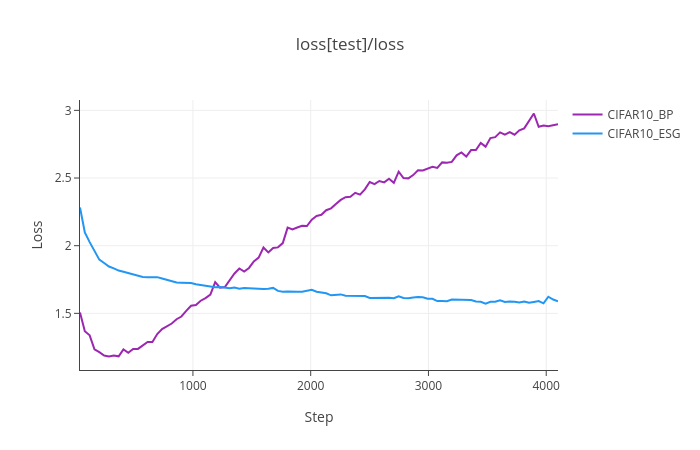
\includegraphics[width=0.7\textwidth]{../report/images/CIFAR10_test.png}
        \caption{CIFAR test}
    \end{figure}      
    \end{column}
% create the column with the second image, that also
% occupies half of the slide
    \begin{column}{.5\textwidth}
    \begin{figure}
        \centering
        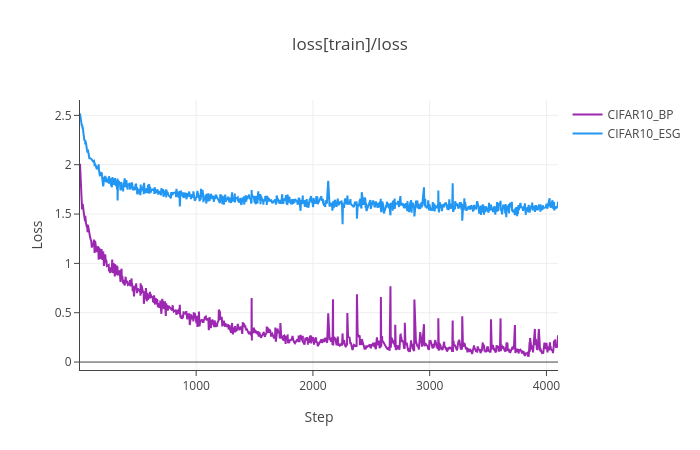
\includegraphics[width=0.7\textwidth]{../report/images/CIFAR10_train.png}
        \caption{CIFAR train}
    \end{figure}
    \end{column}
  \end{columns}

\end{frame}

%------------------------------------------------

\begin{frame}
  \frametitle{MeZo}
  \begin{itemize}
  \item Memory-efficient Zeroth-order
  \item Used for fine-tune huge LLM
  \item Up to 12x memory reduction
  \end{itemize}
  
   \centerline{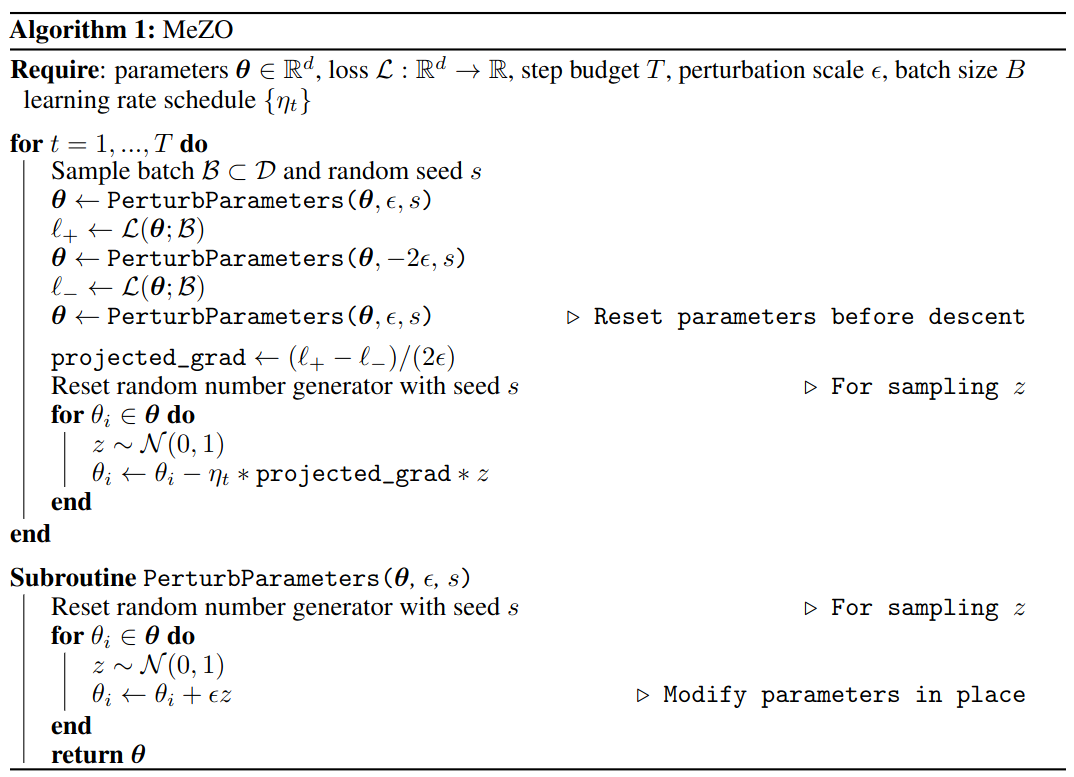
\includegraphics[width=0.6\columnwidth]{../report/images/mezo_alg.png}}
\end{frame}

%----------------------------------------------------------------------------------------
%	CLOSING SLIDE
%----------------------------------------------------------------------------------------

\begin{frame}% The optional argument 'plain' hides the headline and footline
	\begin{center}
		{\Huge The End}
		
		\bigskip\bigskip % Vertical whitespace
		
		{\LARGE Questions? Comments?}
	\end{center}
\end{frame}

%----------------------------------------------------------------------------------------


\end{document} 